\begin{appendices}

\section{Derivation of the reverse acceptance probability}
\label{app:DerivationOfReverseAcceptanceProbability}
If we let $A$ be the event of accepting the proposed transition in the previous HMC step, the probability $\mathbb{P}(A = 1|S_t = s_t, t, x)$ of accepting it given the current position can be related to the distribution of $S_{t-1}^*$ by considering
\begin{equation}
\begin{split}
&\mathbb{P}(A = 1|S_t = s_t, t, x) \\
&\quad= f_{A, S_t|T, X}(1, s_t| t, x)/f_{S_t|T, X}(s_t| t, x),
\end{split}
\end{equation}
where $f_{S_t|T, X}(s_t| t, x) = f_{A, S_t|T, X}(1, s_t| t, x) + f_{A, S_t|T, X}(0, s_t| t, x)$. These terms can then we rewritten using $p_\textrm{accept}(s)$ defined in equation~\eqref{eq:AcceptanceProbability}:
\begin{align}
\begin{split}
&f_{A, S_t|T, X}(1, s_t| t, x) \\
&\quad\qquad = f_{A, S_{t-1}^*|T, X}\big(1, revHD(s_t)| t, x\big) \\
&\quad\qquad = p_\textrm{accept}(revHD(s_t)) \\
&\quad\qquad\qquad \cdot f_{S^*_{t-1}|T, X}\big(revHD(s_t)| t, x\big)
\end{split} \\
\begin{split}
&f_{A, S_t|T, X}(0, s_t| t, x) \\
&\quad\qquad = f_{A, S_{t-1}^*|T, X}\big(0, (z_t, -v_t)| t, x\big) \\
&\quad\qquad = \big(1 - p_\textrm{accept}(z_t, -v_t)\big) \\
&\quad\qquad\qquad \cdot f_{S^*_{t-1}|T, X}\big((z_t, -v_t)| t, x\big)
\end{split}
\end{align}
Now, if $H(z_t, -v_t) \geq H(HD(z_t, -v_t))$ holds, $p_\textrm{accept}(z_t, -v_t) = 1$ and inserting this in the above gives that $\mathbb{P}(A = 1|S_t = s_t, t, x) = 1$. This means the move to $s_t$ must have been accepted.

If this is not the case, then the acceptance probability cannot be simplified further without reducing the flexibility of the model. In this case one would ideally learn an approximation for $\mathbb{P}(A=1|S_t = s_t, t, x)$, taking $s_t$, $x$ and the time point $t$ as inputs. A good starting point for this model can be obtained by assuming that the Markov chain has already converged. Under this assumption $S_{t-1}^*$ would follow the canonical distribution, so we would have $f_{S^*_{t-1}|T, X}(s| t, x) \propto \exp(-H(s))$. Inserting this in the above equations and noting, that $HD(z_t, -v_t) = revHD(z_t, v_t)$ due to the invertibility of HD and $H(z_t, -v_t) = H(z_t, v_t)$ due to the symmetry of the kinetic energy, yields
\begin{equation}
\begin{split}
\mathbb{P}(A = 1&|S_t = s_t, t, x) \\
&= \exp(-H(revHD(s_t)) + H(s_t))
\end{split}
\end{equation}

In a nutshell, if $H(revHD(s_t)) \leq H(s_t)$ holds, the previous move was always accepted. Otherwise, the probability needs to be learnt, but will tend towards $\exp(-H(revHD(s_t)) + H(s_t))$ as the chain converges.

\section{Likelihood estimation by importance sampling}
\label{app:NLLestimateImportSampling}

The marginal likelihood $p(x)$ is estimated using importance sampling by generating $S$ samples from some sampling distribution $p_\textrm{samp}(z|x)$ and using the following estimation:
\begin{equation}
\begin{split}
p(x) &= \E_{z \sim p_\textrm{samp}} \left[\frac{p(x|z) \cdot \pi(z)}{p_\textrm{samp}(z|x)} \right] \\
&\approx \frac{1}{S} \sum_{s=1}^S \frac{p(x|z_s) \cdot \pi(z_s)}{p_\textrm{samp}(z_s|x)} \textrm{ for } z_s \sim p_\textrm{samp}
\end{split}
\end{equation}
For this estimation to be efficient, it is important that the sampling distribution tightly covers the true posterior $p(z|x)$. To achieve this, the sampling distribution, chosen to be a multivariate Gaussian, was centred on an estimate of the mean of the true posterior, obtained by sampling five times from the HMC-enhanced posterior approximation. The covariance matrix was taken from the initial encoder $q_0(z|x)$. This returned low variance estimates of the marginal likelihood with little dependence on the number of samples $S$ for $S > 2000$.

\begin{figure}[hb]
\centering
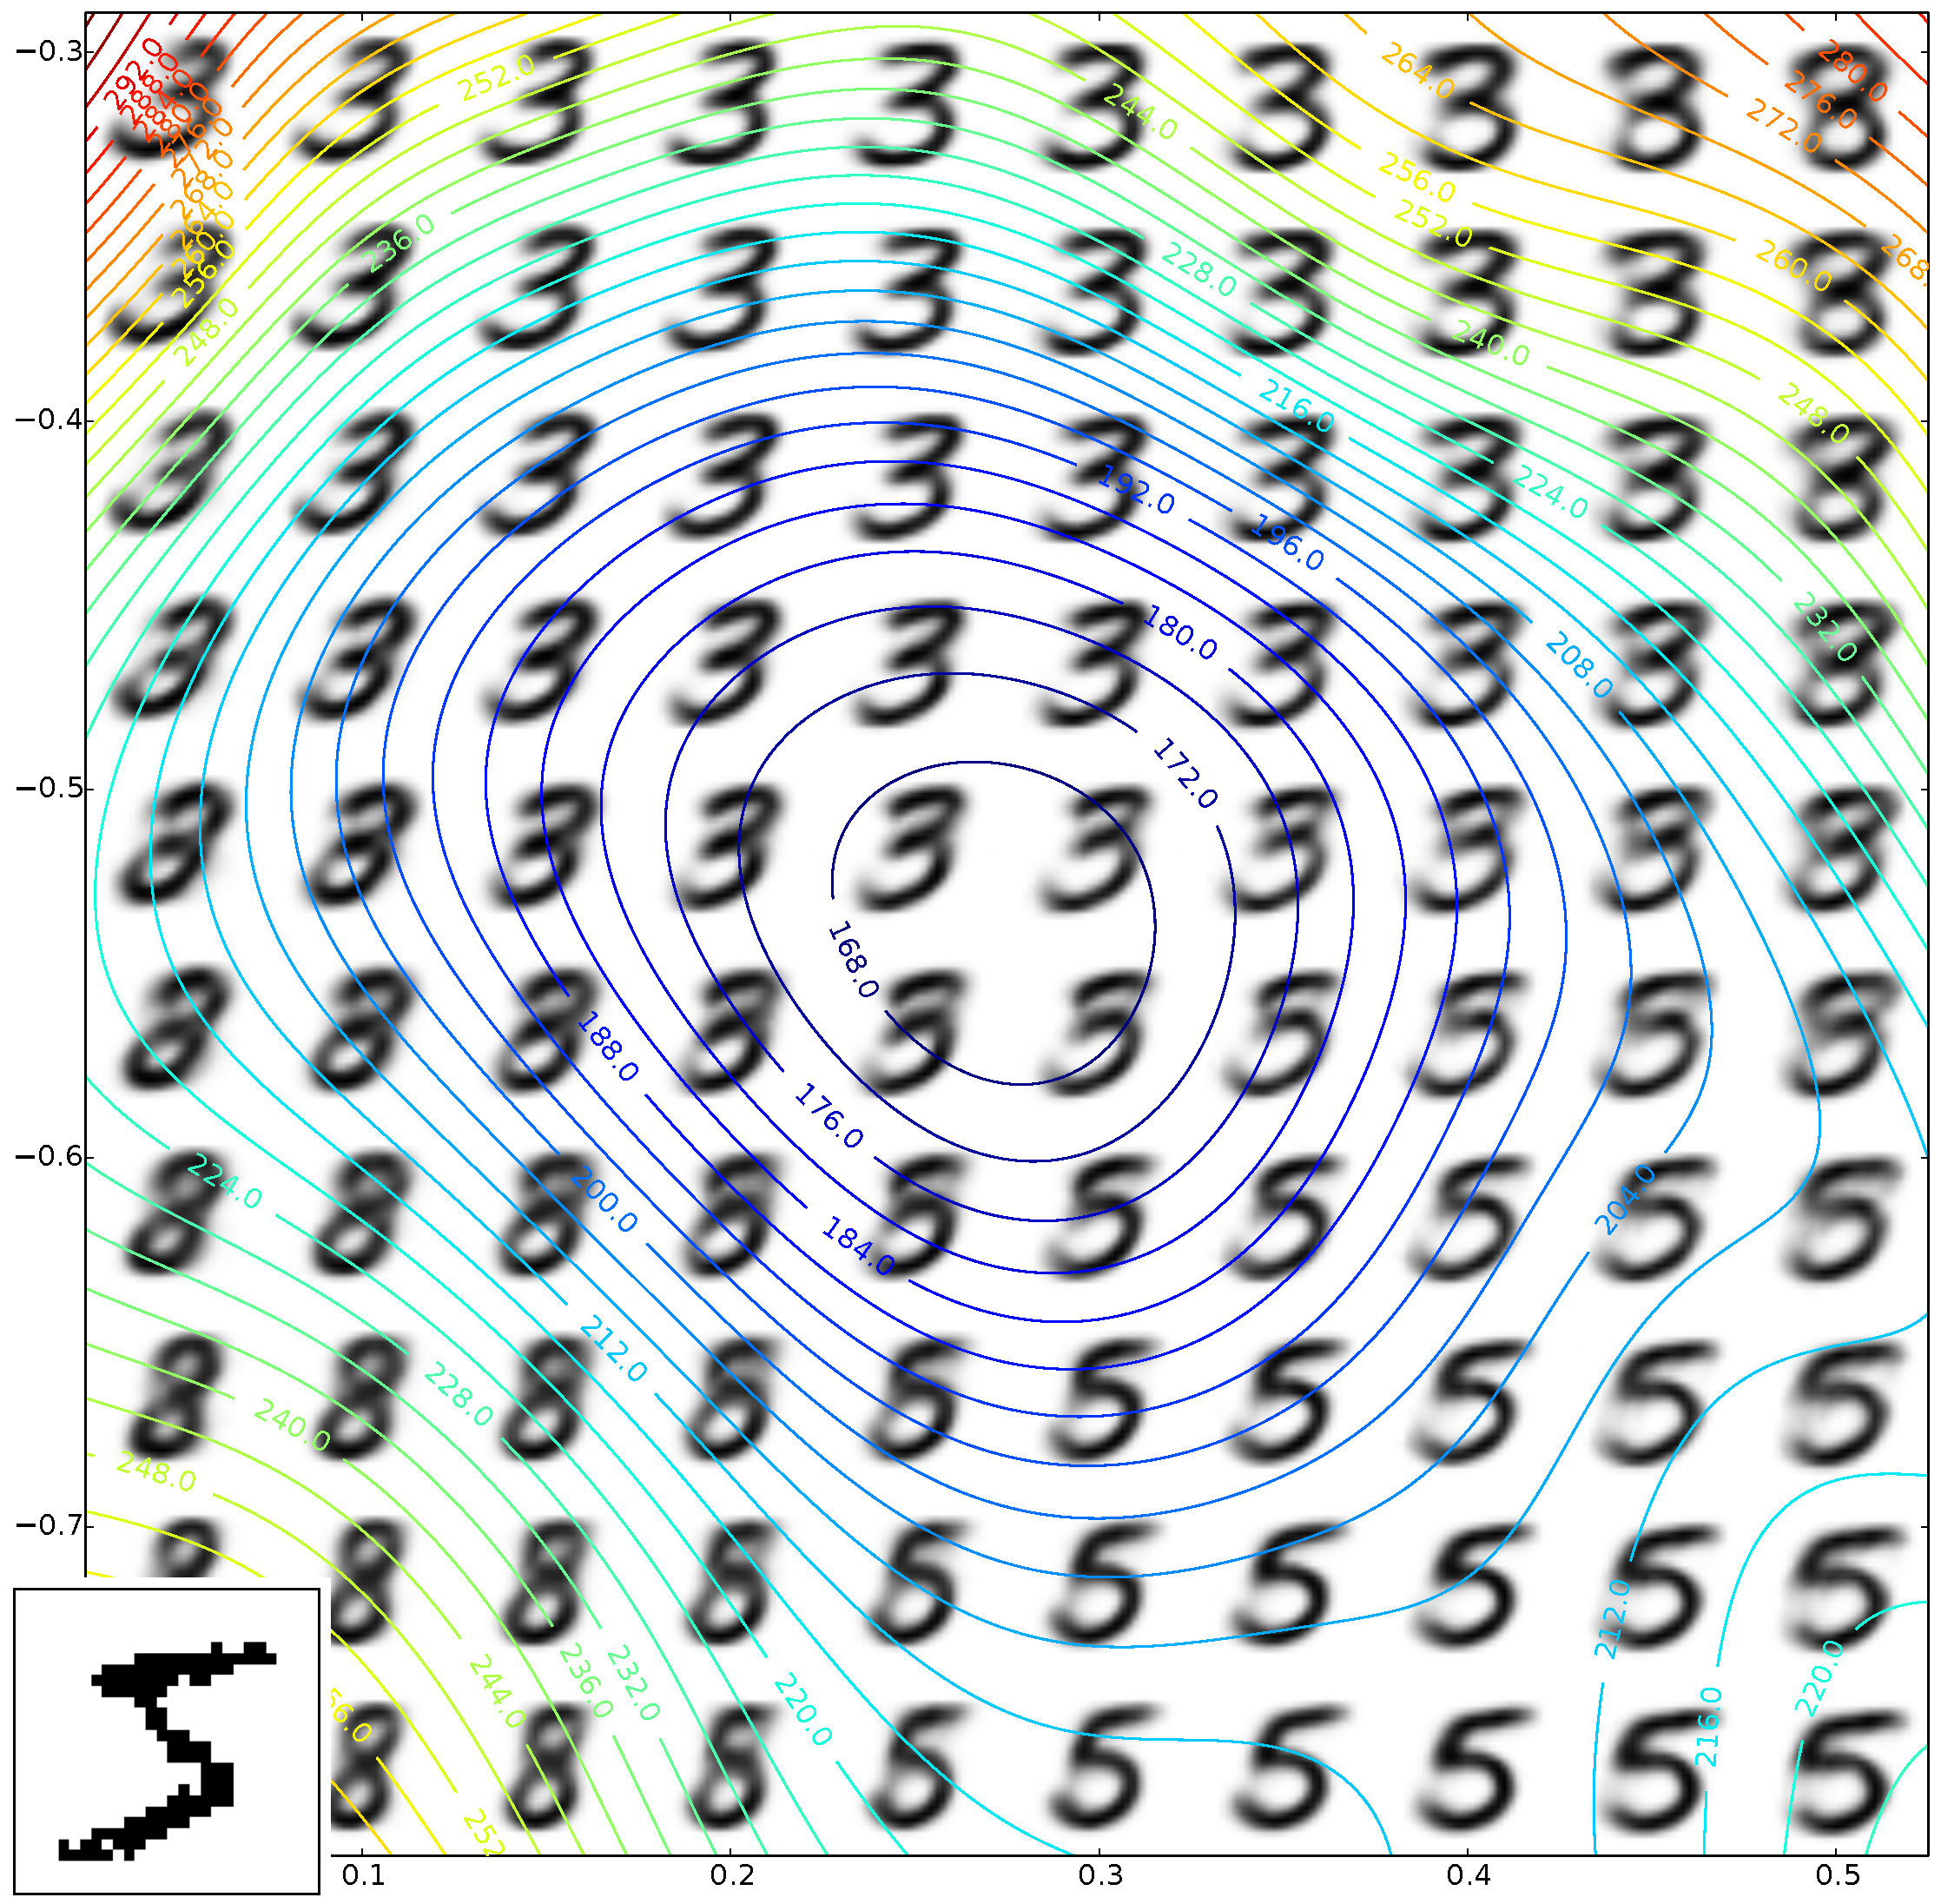
\includegraphics[width=\columnwidth]{figures/vae_pot_energy_example.pdf}
\caption{Potential energy surface for the observed digit shown in the inset. The contours indicate the potential energy surface produced by a trained model with a 2-dimensional latent space. The plot also shows the mean images produced by the decoding model at evenly spaced points of the latent space.}
\label{fig:EnergySurfaceMNIST}
\end{figure}

\section{Visualizations of latent space}
\label{app:LatentVisualizations}

For each MNIST digit $x$ the potential energy surface given by $-\log p(x, z)$ differs. Figure~\ref{fig:EnergySurfaceMNIST} shows the energy surface produced by a trained model for a specific digit. For an intuitive understanding of the potential energy it also shows the mean images produced by the decoding model $p(x|z)$ at evenly spaced points in latent space. The closer the mean image is to the observed digit, the lower the potential energy.

For the best performing model on two-dimensional latent space figure~\ref{fig:2d_latent_visualization} illustrates the learnt latent space, depicting both exemplary mean images produced by the decoding model $p(x|z)$ and the latent space coordinates of the training set under the learnt encoder (including the HMC steps). A clear (but not perfect) separation of the digits is immediately obvious, showing the power of this unsupervised model to capture structures in the data. Interestingly, the latent space is not occupied evenly, with transition areas between the digits completely vacant. With a more flexible decoder this behaviour should become less prominent.

\begin{figure}[hb]
\centering
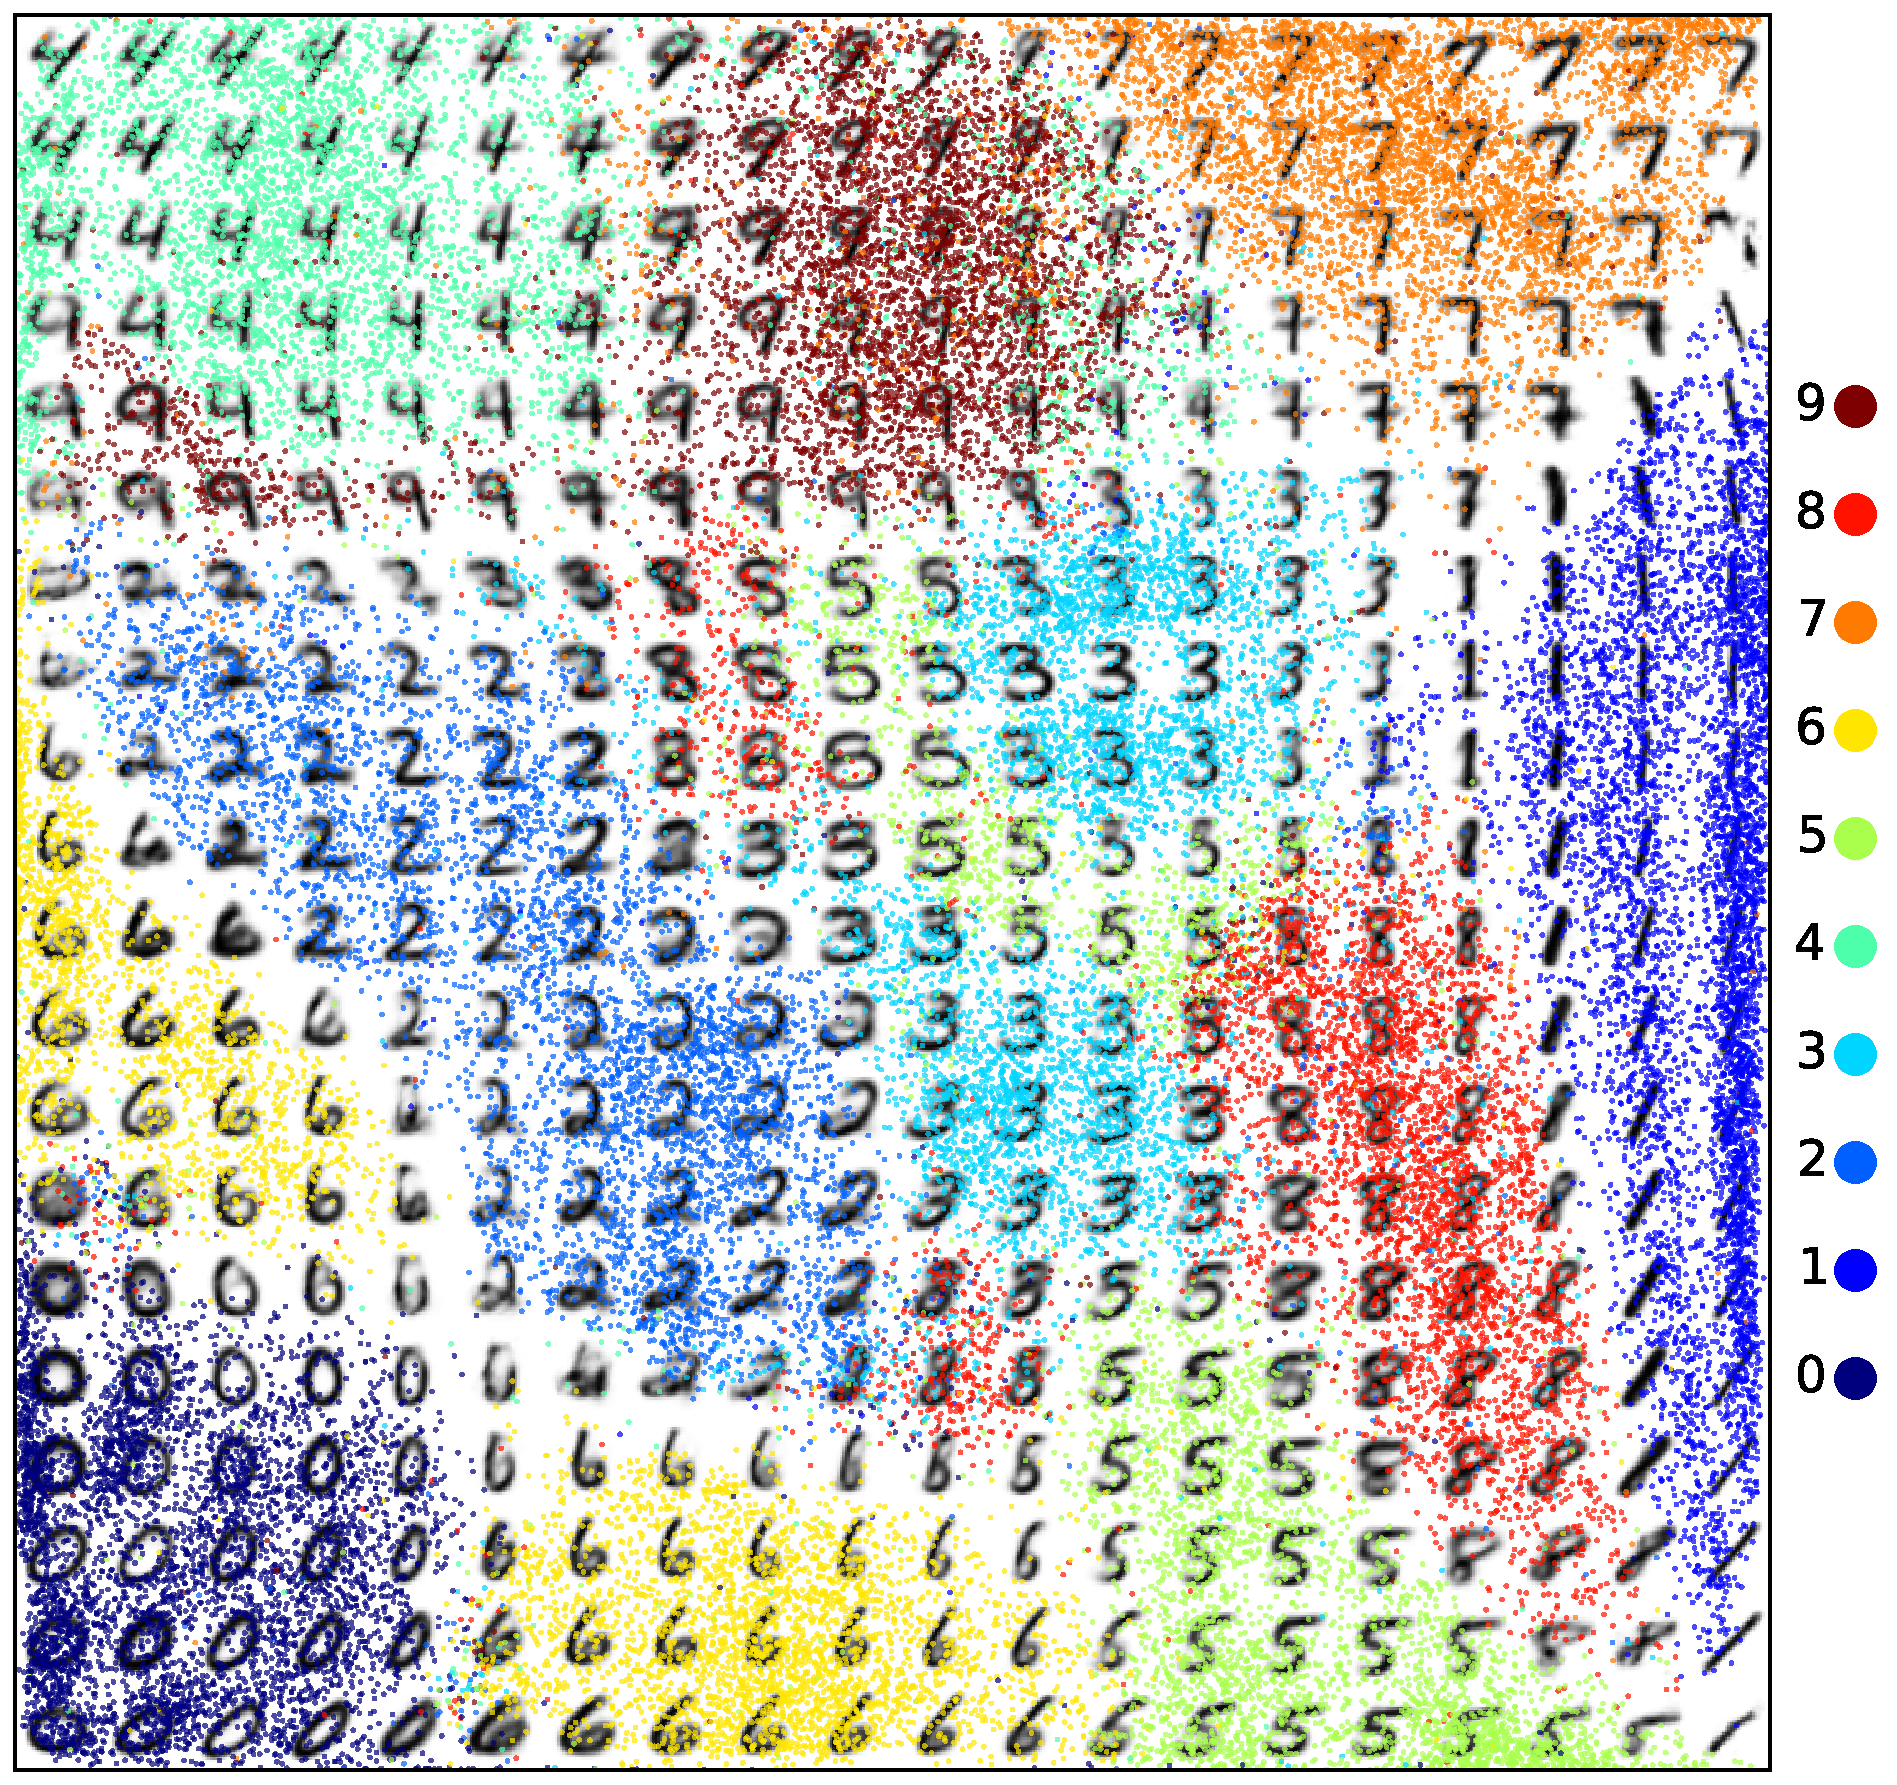
\includegraphics[width=\columnwidth]{figures/learned_representation_train_points_small.pdf}
\caption{Illustration of the two-dimensional latent space representation learnt by the model HMCVI 8 (see table~\ref{tab:Results}). To compensate for the Gaussian prior on the latent variables, linearly spaced coordinates in the unit square were transformed using the inverse Gaussian cdf. Therefore, the prior density in this view of latent space is uniform. For each coordinate the mean image produced by the decoder is shown. Additionally, the latent space representation of the training dataset as produced by the enhanced encoder is depicted (transformed by the Gaussian cdf), where each digit class is indicated by a different color.}
\label{fig:2d_latent_visualization}
\end{figure}

\end{appendices}